\documentclass{beamer}

\mode<presentation> {
  \usetheme{Singapore}
  %\setbeamercovered{transparent}
  %\usecolortheme{wolverine}
}

\usepackage{palatino}
\usepackage{graphicx}
\DeclareMathOperator*{\argmax}{arg\,max}
\newcommand{\test}{\ensuremath{\mathcal{T}}}

\AtBeginSection[]
{
  \begin{frame}
    \frametitle{Table of Contents}
    \tableofcontents[currentsection]
  \end{frame}
}

\title{Identifying License Plates Ids with Hidden Markov
    Models}
\author{ James Pritts and Ondrej Hrstka }
\institute[CTU FEE]{Czech Technical University in Prague - Faculty of Electrical Engineering}
\date{13.2.2012}

\begin{document}
\begin{frame}
  \titlepage
\end{frame}


\section{Introduction}

\begin{frame}
  \frametitle{Problem statement}

\begin{itemize}
\item[Task] Report the unique identifying string of characters, called
  the \emph{vehicle-id}, from the image of a license plate.

\item[Input] Images of license plates that have been segmented and
  ortho-rectified.
\end{itemize}

\end{frame}

\begin{frame}
  \frametitle{Assumptions about data}
\begin{itemize}
\item The font of all characters across license plates is identical.
\item Exemplars of a particular character are the same width (we relax this restriction later).
\item All characters have the same height.
\item There is significant white space between adjacent characters.
\end{itemize}
\end{frame}

\section{Model Definition}
\begin{frame}
  \frametitle{Hidden Markov Model}
\begin{description}
\item[Observations] The left-to-right sequence of consecutive intensity columns from
  the segmented image of the license plate.

\item[Hidden States] The set $\mathbf{K}$ of column
  indexes of all the glyphs in the font set and an added state \texttt{w}
  that represents white-space
\[S =
\left(\,\dots,\texttt{w},\texttt{A}_1,\texttt{A}_2,\ldots,\texttt{A}_{m},\texttt{w},\texttt{w},\texttt{w},\texttt{T}_1,\texttt{T}_2,\ldots\,\right).\]

\item[Emissions] The probabilities of observing pixel
  intensities given their corresponding glyph column, or,
  equivalently, given their \emph{hidden states}.

\end{description}
\end{frame}

\begin{frame}
  \frametitle{Emission Probabilities}

\begin{description}
\item[Row Independence] probabilities of observing intensities in
  a column $\mathbf{x}_j$ are uncorrelated.

  \[p(\mathbf{x}_j \mid s_j) = \prod_{i=1}^np(x_{ij} \mid s_j).\] 

\item[Mixture Model] probability of observing pixel intensity $x_{ij}$
  of a glyph column $s_j$ is modelled as a two-class gaussian mixture.

\[
\mathcal{N}(x_{ij};\sigma_1,\mu_1)\gamma_{is_j}+\mathcal{N}(x_{ij};\sigma_2,\mu_2)(1-\gamma_{is_j})
\]
\end{description} 

**Note that the foreground and background distributions are position
independent.
\end{frame}

\section{Learning the model}

\begin{frame}
  \frametitle{Input dataset}
  Input dataset contains 5000 annotated examples. Each example is structure containing:
\begin{itemize}
  \item Original license plate images
  \item Cropped and normalized image
  \item String with bounding boxes for each character.
\end{itemize}

\begin{figure}
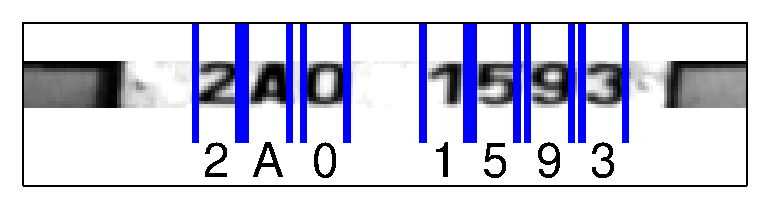
\includegraphics[width=\linewidth]{pics/input_example.eps}
\caption{Example of annotated input data. Normalized image displayed.}
\label{fig:distribution}
\end{figure}

\end{frame}

\begin{frame}
  \frametitle{Difficult data}
\begin{figure}
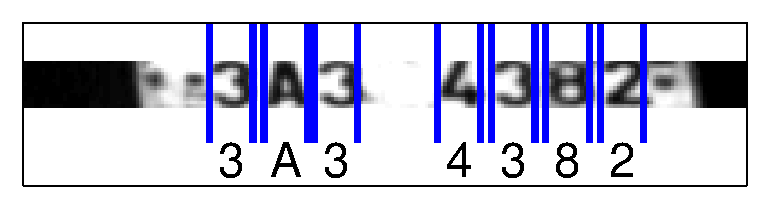
\includegraphics[width=0.8\linewidth]{pics/bad1.eps}
\end{figure}

\begin{figure}
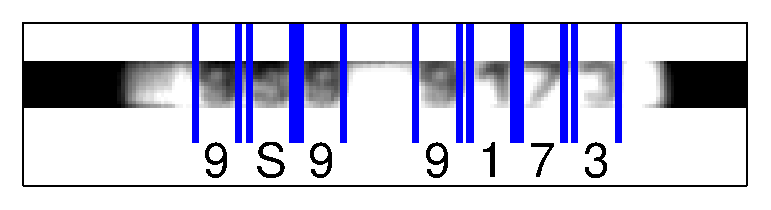
\includegraphics[width=0.8\linewidth]{pics/bad2.eps}
\end{figure}

\begin{figure}
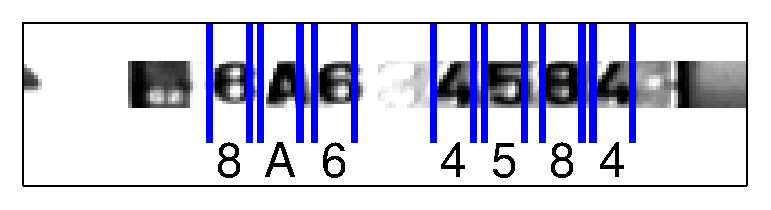
\includegraphics[width=0.8\linewidth]{pics/bad3.eps}
\end{figure}

\end{frame}


\begin{frame}
  \frametitle{Learning the emission probabilities}
  \begin{itemize}
  \item There are no annotations for foreground and background pixels.
  \item Unsupervised learning is required to determine emission probability parameters.
  \item Emission probabilities of the model were learned using \textbf{EM} algorithm.
\end{itemize}
\end{frame}

\begin{frame}
  \frametitle{Learning the emission probabilities}
\begin{block}{E-step}
	\[
  p^{t+1}( c=f \mid x^d_{ij}, s_j) =
  \frac{\mathcal{N}(x^d_{ij};\sigma_1^t,\mu_1^t)\gamma_{is_j}^t}{\mathcal{N}(x^d_{ij};\sigma_1^t,\mu_1^t)\gamma_{is_j}^t+\mathcal{N}(x^d_{ij};\sigma_2^t,\mu_2^t)(1-\gamma_{is_j}^t)}
\]
	\end{block}

\begin{block}{M-step}
\[
  \gamma_{is_j}^{t+1} = \frac{\sum_{d \in \mathcal{D}} p^{t+1}( c=f \mid x^d_{ij}, s_j)}{\sum_{d \in \mathcal{D}} p^{t+1}( c=f \mid x^d_{ij}, s_j)+ \sum_{d \in \mathcal{D}} (1-p^{t+1}( c=f \mid x^d_{ij}, s_j))}
\]
\[
  \mu_1^{t+1} = \frac{\sum_{i,j} \sum_{d \in \mathcal{D}} x^d_{
      ij} p^{t+1}( c=f \mid x^d_{ij}, s_j)}{\sum_{i,j} \sum_{d \in
      \mathcal{D}} p^{t+1}( c=f \mid x^d_{ij}, s_j)}
\]
\end{block}  
\end{frame}

\begin{frame}
  \frametitle{Learning the emission probabilities}
\begin{itemize}
\item Stopping criterion is relative
\item  $|1-\frac{\mu_1^{t+1}}{\mu_1^{t}}| < \epsilon \wedge
|1-\frac{\mu_2^{t+1}}{\mu_2^{t}}| < \epsilon$
\item$\epsilon$ has been set to value $10^{-5}$
\end{itemize}  
\end{frame}

\begin{frame}
  \frametitle{Learned templates}
\begin{figure}[htp]
\centering
\includegraphics[width=\linewidth]{pics/jba.png}
\caption{Learned templates of \texttt{J}, \texttt{B} and
  \texttt{A}. Intensity corresponds to the prior probability for being
  a foreground pixel.}
\label{fig:templates}
\end{figure}
\end{frame}

\begin{frame}
  \frametitle{Setting the transition probabilities}
\begin{itemize}
\item Permitted transitions were set by hand and derived qualitatively
  from the data
\item Transitions include white-space to white-space, white-space to
  first glyph columns, between consecutive glyph columns, between
  terminal glyph columns and white-space.
\item allow transitions to the same glyph column. Transitions to
  non-consecutive glyph columns and from non-terminal glyph columns to
  white-space are prohibited.
\end{itemize}

The white-space to white-space transitions can be calculated as follows

\[ 
 p(s_i=\text{w} \,|s_{i-1}=\text{w}) = 2-\sqrt{\frac{4}{E[W]}}.
\]
\end{frame}


\begin{frame}
  \frametitle{Inference}
\begin{itemize}
\item  The hamming loss function is used for risk assessment.
\item HMM contains transitions with zero probabilities. 
\item  Finding a valid sequence of hidden states that minimizes risk
under the hamming loss is equivalent to minimizing the expected
hamming loss over the subset of hidden states that have non-zero
transitions.  
\[ 
\argmax_{s \in \rho} \sum_{i=1}^n p(x,s_i) \qquad \text{where } \rho =
       \{\, s \mid p(s) > 0 \,\} \subset K^n
\]
\item Inference algorithm is $\mathcal{O}(2|K|^2n)$ + $\mathcal{O}(|K|n)$
\end{itemize}
  
\end{frame}

\section{Evaluation}
\begin{frame}
  \frametitle{Good results}

\begin{figure}
  \centering
  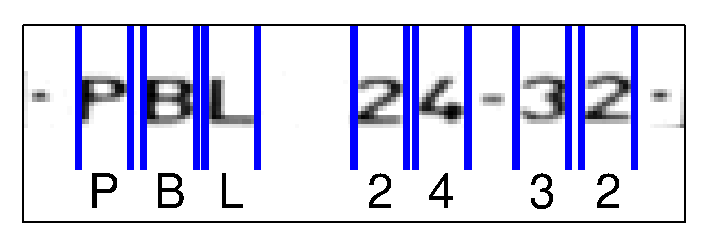
\includegraphics[width=0.6\textwidth]{pics/lic_PBL2432.eps}          
\end{figure}  
  
\begin{figure}
  \centering
  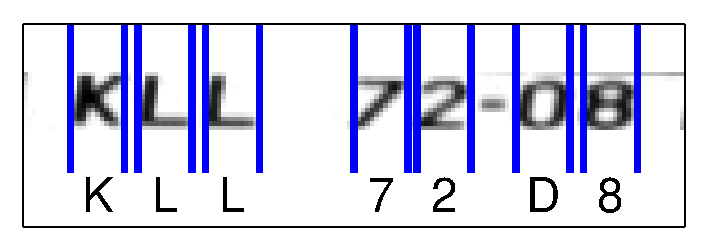
\includegraphics[width=0.6\textwidth]{pics/lic_KLL72D8.eps}
\end{figure}  

\begin{figure}
  \centering
  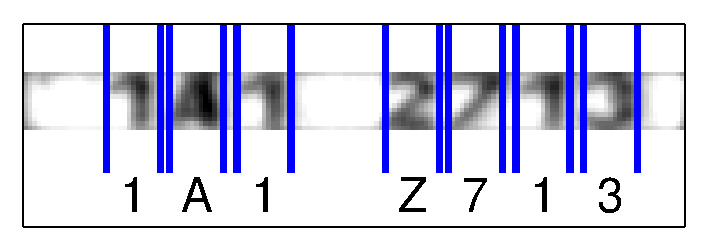
\includegraphics[width=0.6\textwidth]{pics/lic_1A1Z713.eps}
\end{figure}    
  
\end{frame}

\begin{frame}
  \frametitle{Segmentation metric}
\begin{description}
\item[correct segmentation] occurs when an \emph{inferred character
  region} sufficiently overlaps an \emph{annotated character region}
\item[overlap]
\[
\left|1-\frac{|R^k_i \cap \hat{R}^k_j|}{|R^k_i|}\right| < 0.15
\]   
\item[prob of detection] ($p_d$) the ratio of correct segmentations to
  the total number of annotated character regions in the test set.
\item[prob of false alarm] ($p_{fa}$) the ratio of annotated
  white-space regions that are inferred as character regions to the
  total number annotated white-space regions.
\end{description}
\end{frame}

\begin{frame}
  \frametitle{Segmentation performance}
  \begin{table}[ht]
    \begin{center}
      \begin{tabular}{|l|l|}
        \hline
        \multicolumn{2}{|c|}{Segmentation Performance} \\
        \hline
        $p_d$ & 71.9\% \\
        $p_{fa}$ & 7.60\% \\
        \hline
      \end{tabular}
      \caption{Calculated for \texttt{np-images-5000.mat}}
      \label{table:segmentation}
    \end{center}
  \end{table}
\end{frame}

\begin{frame}
\frametitle{Inference accuracy}
\begin{description}
\item[Levenshtein distance] minimum number of edits needed to transform one string into the
other, with the allowable edit operations being insertion, deletion,
or substitution of a single character.

\[ \text{accuracy} = \frac{\sum_{k \in \test}
  d_L(\hat{id}_k,id_k)}{7|\test|} \qquad \test \text{ is test set }  \]
\end{description}

\begin{table}[ht]
\begin{center}
\begin{tabular}{|l|l|}
  \hline
  \multicolumn{2}{|c|}{ID accuracy} \\
  \hline
  $accuracy$ & 36.5\% \\
  \hline
\end{tabular}
\caption{Calculated for \texttt{np-images-5000.mat}}
\end{center}
\end{table} 
  
\end{frame}

\begin{frame}
  \frametitle{Levenshtein distance}
  \begin{figure}
\begin{center}
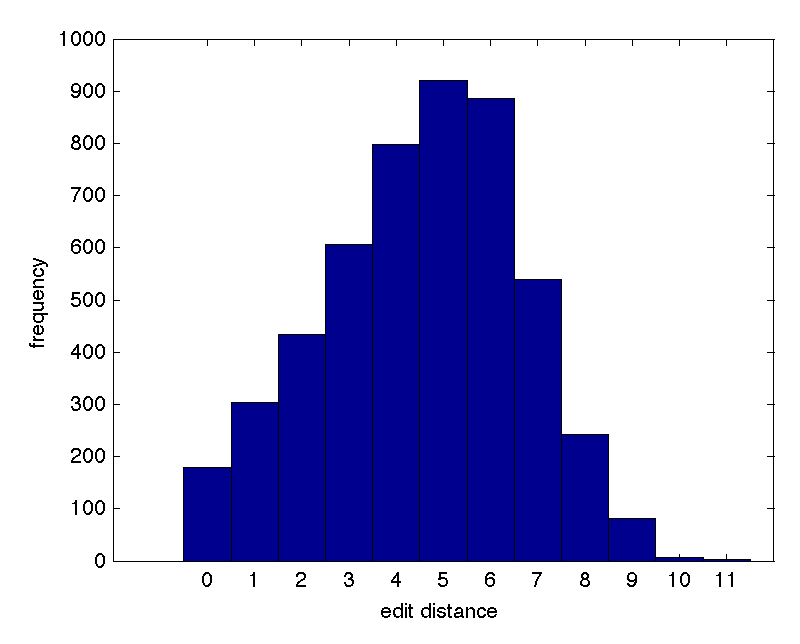
\includegraphics[width=0.75\linewidth]{pics/hamming.eps}
\caption{ Frequency of edit distance over \texttt{np-images-5000.mat}  } 
\label{fig:editdistance}
\end{center}
\end{figure}
\end{frame}

\begin{frame}
  \frametitle{Identified Problems}
\begin{itemize}
\item not suitable for operational use.
\item throwing away problematic annotations means that our templates
  are not be representative of some of the badly conditioned data.
\item prohibited non-zero transitions to non-consecutive glyph
  columns.
\item The transition model does not account for cases where there is
  no apparent white space between characters.
\item did not create a template for hyphens which occur in a
  significant number of the license plates.
\item Need supervised learning
\item There as a large overlap and large variance of the global
  intensity models (see Figure \ref{fig:distribution}) estimated
  during training.
\item no explicit model created for the license plate string.
\end{itemize}
\end{frame}

\end{document}
